\documentclass[a4paper, 8pt, oneside]{article}

 \usepackage[margin=1in]{geometry} 
\usepackage{amsmath,amsthm,amssymb, float,centernot}
\usepackage[shortlabels]{enumitem}
 \usepackage[hidelinks]{hyperref}
\usepackage{xcolor}
\usepackage{graphicx}
\usepackage[T1]{fontenc}
\hypersetup{
    colorlinks,
    linkcolor={red!50!black},
    citecolor={blue!50!black},
    urlcolor={blue!80!black}
}
\newcommand{\arcangle}{\mathord{\mathpalette\doarcangle\relax}}
\newcommand{\doarcangle}[2]{%
  \hbox{%
    \sbox0{$#1B$}%
    \sbox2{$#1<$}%
    \raisebox{\dimexpr\dp2+(\ht0-\ht2)/2}{%
      $#1<\mspace{-9mu}\mathrel{)}\mspace{2mu}$%
    }%
  }%
}

\newtheorem{theorem}{Theorem}[section]
  
\newcommand{\N}{\mathbb{N}}
\newcommand{\Z}{\mathbb{Z}}
\newcommand{\R}{\mathbb{R}}
\newcommand\abs[1]{\left|#1\right|}
\newenvironment{sol}
    {\emph{Solution:}
    }
    {
    \qed
    }
    


\begin{document}

\title{Computational Geometry: Assignment 2}
\author{Oren Friman 301677613}
\maketitle

\medskip

\begin{enumerate}
\item \label{item:q1} Describe in detail an algorithm that solves in  $\mathcal{O}(n\log{}n)$ time the following problem: \\
Input:
 \begin{itemize}
  \item A collection on $n$ disjoint segments in the plane $s_1, \ldots, s_n$ each one given by its two endpoints.
  \item A point $p$ in the plane, not lying on any segment.
\end{itemize}
Output: The set $\{ i \mid s_i \text{ is visible from } p\}$ \\
A segment $s_i$ is visible from $p$ if there exists a point $q \in s_i$ such that the segment $pq$ does not intersect  any other segment $s_j$. In the following example, the segments visible from $p$ are colored blue and the other ones are colored red:
\begin{figure}[h]
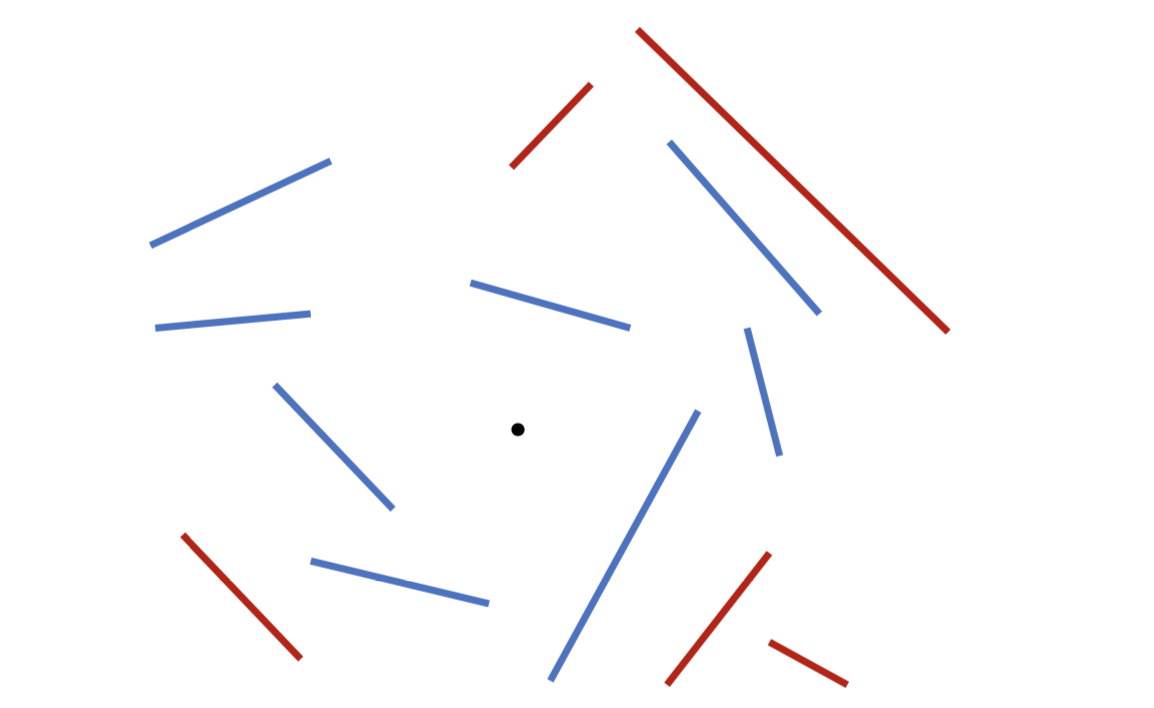
\includegraphics[scale=0.5]{example1}
\centering
\end{figure} \\
You can assume general position for simplicity. \\
\textbf{Hint:} Use a radial sweep centered at $p$. \\ \\
\begin{sol}

The plane sweep algorithm  presented in the class and in the book \cite[Chapter 2]{computationalbook} used a horizontal line to sweep downwards over the plane. For this problem it will be more convenient to sweep the plane with a rotating line (radial sweep centered at $p$).

We start by describing the data structures the algorithm uses -
 \begin{itemize}
   \item Event queue $\mathcal{Q}$, balanced binary search tree, 
   the queue will allow to get the next event ordered by $\prec$ and remove it from the queue.
   Define an order $\prec$ on the events points - if $e_1$ and $e_2$ are two event points and $\ell$ is the sweep line then we have $e_1 \prec e_2$ if and only if $\arcangle (e_1 p) \ell > \arcangle (e_2 p) \ell$ holds or $\arcangle (e_1 p) \ell = \arcangle (e_2 p) \ell$ and distance$(e_1, p)$ $<$ distance$(e_2, p)$ holds.
  \item Status structure $\mathcal{T}$, balanced binary search tree that contain ordered sequence of segments intersecting the sweep line.
\end{itemize}

\textbf{Algorithm} FINDVISIBLE$(S, p$)\\
\textit{Input}:
 \begin{itemize}
  \item A collection on $n$ disjoint segments in the plane $s_1, \ldots, s_n$ each one given by its two endpoints.
  \item A point $p$ in the plane, not lying on any segment.
\end{itemize}
\textit{Output}. The set $\{ i \mid s_i \text{ is visible from } p\}$ \\
\begin{enumerate}
\item Initialize an empty event queue $\mathcal{Q}$. Next, insert the segment endpoints into $\mathcal{Q}$, the corresponding segment should be stored with it.
\item Initialize an empty status structure $\mathcal{T}$.
\item \quad \textbf{while} $\mathcal{Q}$ is not empty
\item \quad \quad \textbf{do} Determine the next event point $q$ in $\mathcal{Q}$ and delete it. HANDLEEVENTPOINT($p, q$)
\end{enumerate}

\textbf{Algorithm} HANDLEEVENTPOINT$(p, q$)\\
\begin{enumerate}
\item if $q$ is left point in the segment insert the segment to $\mathcal{T}$ else delete $q$ segment from $\mathcal{T}$.
\item the closet segment $s_i$ in $\mathcal{T}$ to $p$ is visible.
\end{enumerate}
Time complexity analysis - \\
Constructing the event queue is $\mathcal{O}(n\log{}n)$ \\
 iterate over all events $\mathcal{O}(n)$ and for each we update $\mathcal{T}$ which take $\mathcal{O}(\log{}n)$. \\
 So we get $\mathcal{O}(n\log{}n)$.
\end{sol}

\item \label{item:q2}  Recall that a polygon $\mathcal{P}$ is called y-monotone if every horizontal line  intersects $\mathcal{P}$ in at most two points. \\
\begin{figure}[h]
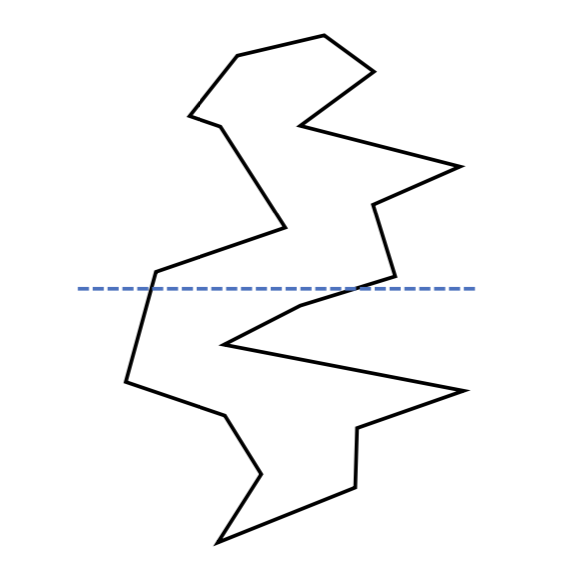
\includegraphics[scale=0.5]{example2}
\centering
\end{figure} \\
Given a line $\ell$, call a polygon $\mathcal{P}$ $\ell$-monotone if every line perpendicular to $\ell$ intersects $\mathcal{P}$ in at most two points. \\ 

Describe in detail an efficient algorithm that, given a polygon $\mathcal{P}$ with $n$ vertices, determines whether there exists a line $\ell$ such that $\mathcal{P}$ is $\ell$-monotone. What is the running time of your algorithm?\\

\begin{sol}
Given a polygon $\mathcal{P}$ with $n$ vertices $\{v_1, \ldots, v_n \}$ - \\

 \begin{enumerate}
   \item  \label{itm:setp1}  Let $v_l$ and $v_r$ be the  vertices with the min and max  x-coordinate value  respectively(exhaustive search).\\
         \begin{minipage}{\linewidth}
            \centering
            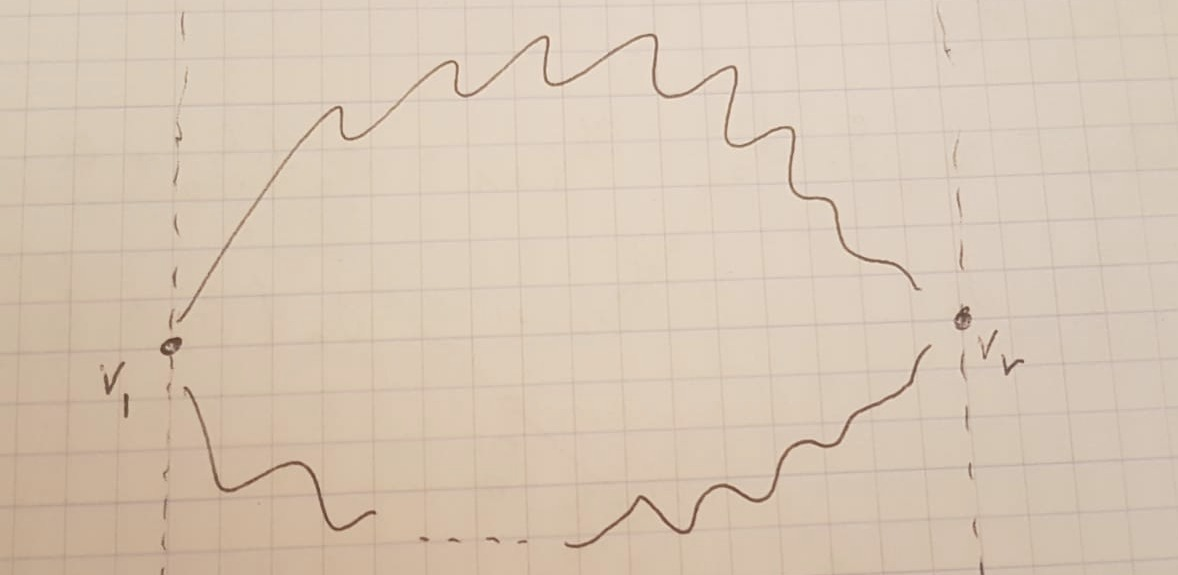
\includegraphics[scale=0.2]{chanis}
        \end{minipage} \\
\item \label{itm:setp2} return true if all  x-coordinate values in  $v_l, v_{l+1\%n}, v_{l+2\%n}, \ldots, v_r$ and $v_l, v_{l-1\%n}, v_{l-2\%n}, \ldots, v_r$ are not decreasing.\\

This way we avoid bad cases -\\
      \begin{minipage}{\linewidth}
            \centering
            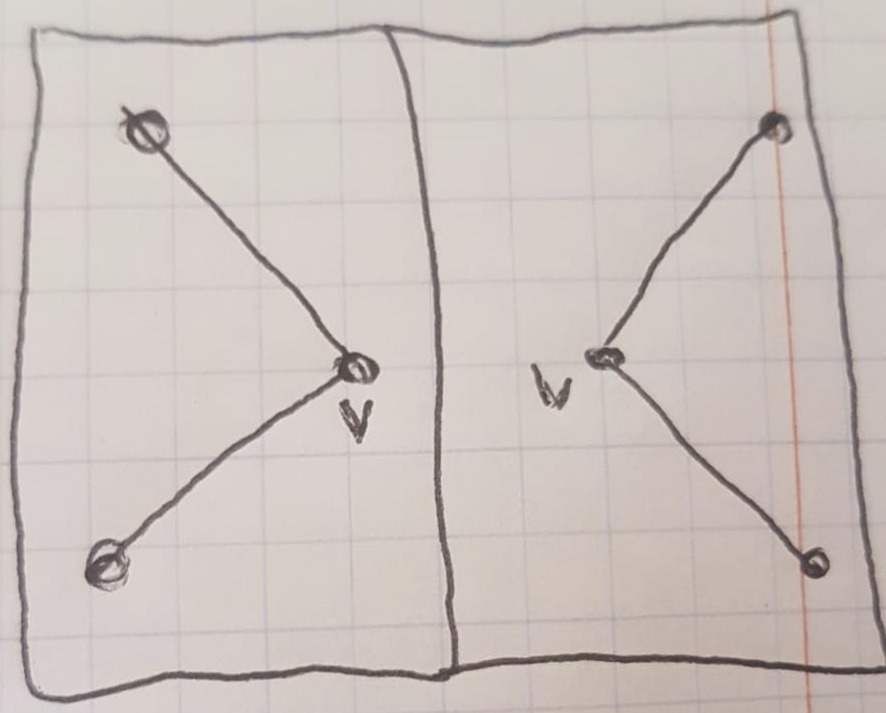
\includegraphics[scale=0.2]{ver}
        \end{minipage} \\
\end{enumerate}
Notice that we iterate over all vertices in (\ref{itm:setp1}) $\mathcal{O}(n)$ and iterate over the sequences in (\ref{itm:setp2}) $\mathcal{O}(n)$  so we get that the time complexty is $\mathcal{O}(n)$.
\end{sol}
\item Recall that, in the incremental construction of the trapezoidal decomposition induced by a set of segments, we maintain a “history DAG” G that stores all trapezoids that ever existed. The insertion order of the segments is very significant, because it affects the number of nodes in G, as well as the length of the longest path in G.\\ \\
Give an example of a set of $n$ segments, as well as an insertion order for them, that causes G to have $\mathcal{O}(n^2)$ nodes and a root-to-sink path of length $\mathcal{O}(n)$. \\

\begin{sol} \\ 
	Let the insertion order of $n$ segments be as follows (the order is by the segment index) -\\
      \begin{minipage}{\linewidth}
            \centering
            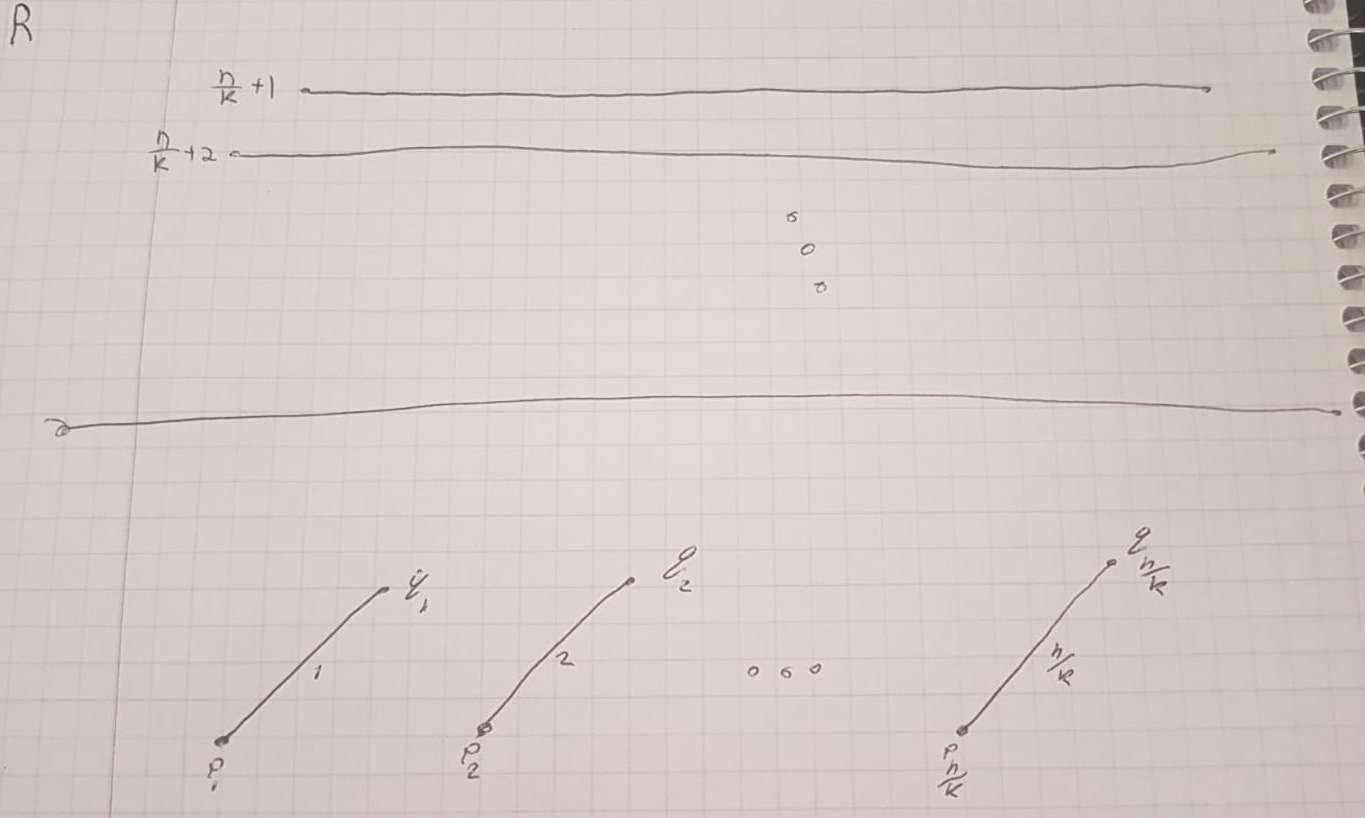
\includegraphics[scale=0.2]{line}
        \end{minipage} \\
        Where $k \in \mathcal{O}(1)$.\\
        \textbf{depth} - each iteration where $1 \leq i \leq \frac{n}{k}$ will add 2 to the maximum depth so after the first $ \frac{n}{k}$ iterations a root-to-sink path is $\mathcal{O}(n)$.\\
           \begin{minipage}{\linewidth}
            \centering
            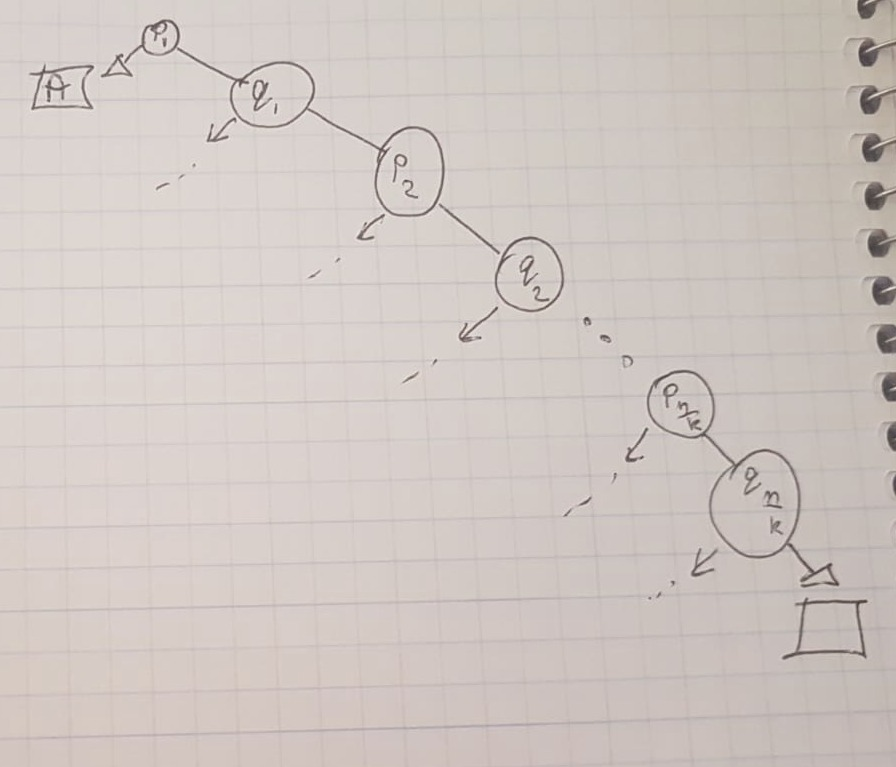
\includegraphics[scale=0.2]{dag}
        \end{minipage} \\
         \textbf{nodes} - each iteration where $i > \frac{n}{k}$, will remove $\mathcal{O}(n)$ trapezoids so each iteration will update the DAG and create those new leaves, there will be $\mathcal{O}(n)$ iterations where $i > \frac{n}{k}$ so there will be $\mathcal{O}(n^2)$ nodes in the history DAG (search structure).
\end{sol}
\end{enumerate}


\medskip
 
\begin{thebibliography}{9}
\bibitem{computationalbook} 
Mark de Berg, Otfried Cheong, Marc van Kreveld, Mark Overmars.
\textit{Computational Geometry: Algorithms and Applications 3rd Edition}, 2008.
\end{thebibliography}

\end{document}